\documentclass[letterpaper, 12pt]{article}
\usepackage{graphicx} % Required for inserting images
\usepackage{textcomp}
\usepackage{fullpage}
\usepackage{amsmath}
\usepackage{xcolor}
\usepackage{float}
\usepackage{enumitem}
\usepackage{geometry}
\geometry{margin=1in}
\usepackage{enumitem}
\usepackage{hyperref}
\usepackage{microtype}
\usepackage{gensymb}
\usepackage{parskip}
\usepackage{tikz}
\usepackage{pgfplots}
\pgfplotsset{compat=1.18}
\usepackage{nicefrac}
\hypersetup{
    colorlinks=true,        % Enable colored links
    linkcolor=teal,         % Set color for internal links
    citecolor=teal,         % Set color for citations
    filecolor=teal,         % Set color for file links
    urlcolor=teal           % Set color for URLs
}

\DeclareMathOperator{\arcsec}{arcsec}

\newcommand{\example}[1]{\textcolor{blue}{\textbf{Example:} #1}}
\newcommand{\step}[2]{\textcolor{blue}{\textbf{Step #1:} #2}}

\begin{document}

\begin{center}
\textbf{{\Large AP Calculus BC Test 3}}
\end{center}

\subsection*{H20 Slope fields and Euler's method}

A slope field is a graphical representation of a differential equation that shows the slope of the solution curve at each point in the plane.

For example, the slope field for the differential equation $\displaystyle \frac{dy}{dx} = x^2 - x -2$ can be drawn by calculating the slope at various points $(x, y)$ and drawing small line segments with those slopes. The result is (from Wikipedia):

\begin{figure}[H]
\centering
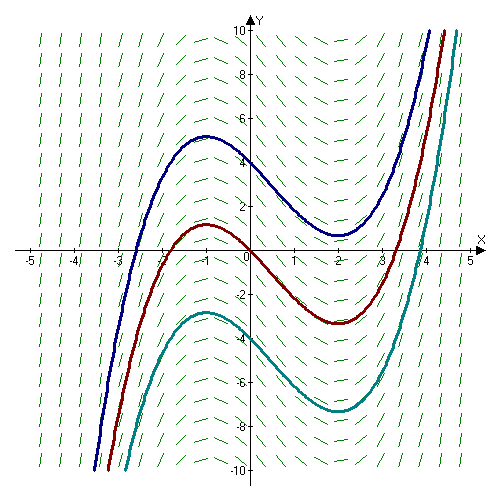
\includegraphics[width=0.5\textwidth]{slopefield.png}
\end{figure}

Euler's method is a technique used to approximate solutions to differential equations with a given initial value by using the slope of the function at a given point to estimate the value of the function at the next point.

\example{Use a table and Euler's method to approximate the value of $y$ at $x=1$ for the differential equation $\displaystyle \frac{dy}{dx} = x + y$ with the initial condition $y(0) = 1$, using a step size of $h=0.5$. Use $\Delta y = \displaystyle \frac{dy}{dx} \cdot \Delta x$ to find the change in $y$ at each step.}

\step{1}{Make a table with the initial condition and known values.}

\begin{table}[H]
\centering
\begin{tabular}{|c|c|c|c|c|c|}
\hline
$x$ & $y$ & $\Delta x$ & $\frac{dy}{dx} = x + y$ & $\Delta y$ & $(x + \Delta x, y + \Delta y)$ \\
\hline
0 & 1 & 0.5 & - & - & $(0.5, y)$ \\
0.5 & - & 0.5 & - & - & $(1, y)$ \\
\hline
\end{tabular}
\end{table}

\step{2}{Calculate the slope $\displaystyle \frac{dy}{dx}$ at each point and use it to find $\Delta y$.}

\begin{table}[H]
\centering
\begin{tabular}{|c|c|c|c|c|c|}
\hline
$x$ & $y$ & $\Delta x$ & $\frac{dy}{dx} = x + y$ & $\Delta y$ & $(x + \Delta x, y + \Delta y)$ \\
\hline
0 & 1 & 0.5 & 1 & 0.5 & $(0.5, 1.5)$ \\
0.5 & 1.5 & 0.5 & 2 & 1 & $(1, 2.5)$ \\
\hline
\end{tabular}
\end{table}

\example{Use tangent lines to do the same problem.}

\step{1}{Find the equation of the tangent line at the initial point.}

Given:

\begin{gather*}
\frac{dy}{dx} = x + y \\
y(0) = 1 \\
\Delta x = 0.5
\end{gather*}

Finding the tangent line:

\begin{gather*}
\frac{dy}{dx} = 0 + 1 = 1 \\
y - 1 = 1(x - 0) \\
y = x + 1
\end{gather*}

\step{2}{Use the tangent line to approximate $y$ at $x=0.5$.}

At $x=0.5$, $y = 0.5 + 1 = 1.5$.

\step{3}{Use the new point to find the next tangent line.}

\begin{gather*}
\frac{dy}{dx} = 1.5 + 0.5 = 2 \\
y - 1.5 = 2(x-0.5) \\
y = 2x + 0.5
\end{gather*}

\step{4}{Use the new tangent line to approximate $y$ at $x=1$.}

At $x=1$, $y = 2(1) + 0.5 = \boxed{2.5}$.

Both methods yield the same approximation of $y(1) \approx 2.5$.

\subsection*{H21 Separable differential equations}

A separable differential equation is one that can be expressed in the form $\frac{dy}{dx} = f(x)g(y)$, allowing the variables to be separated on opposite sides of the equation for integration.

\example{Solve the separable differential equation $\displaystyle \frac{dy}{dx} = \frac{x}{y}$ with the initial condition $y(0) = 2$.}

\step{1}{Separate the variables.}

\begin{gather*}
\frac{dy}{dx} = \frac{x}{y} \\
y \: dy = x \: dx
\end{gather*}

\step{2}{Integrate both sides to find the general solution.}

\begin{gather*}
\int y \: dy = \int x \: dx \\
\frac{1}{2} y^2 = \frac{1}{2} x^2 + C \\
y^2 = x^2 + C \\
\end{gather*}

\step{3}{Use the initial condition to find the particular solution.}

\begin{gather*}
y^2 = x^2 + C\\
y(0) = 2 \\
2^2 = 0^2 + C \\
C = 4 \\
y = \pm \sqrt{x^2+4} \\
2 = \pm \sqrt{0^2 + 4} \\
2 = \sqrt{4} \\
\boxed{y = \sqrt{x^2 + 4}}
\end{gather*}

\subsection*{H22 Logistic equations}

A logistic equation is a type of differential equation that models population growth with a carrying capacity.

Typically, the logistic equation is expressed as $$\frac{dP}{dt} = kP(M-P)$$

where $P$ is the population size, $k$ is the growth rate, and $M$ is the carrying capacity.

Important things to note:
\begin{itemize}
\item The population grows fastest at $P = \displaystyle \frac{M}{2}$, or in the middle of the curve at the point of inflection.
\item As $P$ approaches $M$, the growth rate slows down and the population stabilizes. The rate of change approaches zero as the population approaches its carrying capacity.
\item If the equation is not in the standard form, it may need to be manipulated algebraically to identify $k$ and $M$.
\end{itemize}

\end{document}